\section{Pathway Browser Implementation}
\label{sect:maw_implementation}

\mawapp must track a few different categories of data. The most basic is a
representation of the data model of the online PathCase MAW database, derived
from the web service interface to the database. Examples include pathways,
metabolites, compartments, and processes. In Model-View-Controller terms (see
\ref{sect:cocoa_mvc}), these are \textbf{model} classes.  These model
objects are rendered in \textbf{views}, such as the main pathway graph view.
The models and views are managed by \textbf{controllers} which manipulate the
models and configure the views.

The relationships between some of the major classes of \mawapp are represented
in three figures. Figure \ref{fig:maw_components} shows references between
instances. Figure \ref{fig:maw_controlflow} shows the flow of control in
response to events from the event loop. Figure \ref{fig:maw_dataflow} shows the
flow of data between the methods involved in loading and displaying a graph.

\subsubsection{User Interface}
\label{sect:maw_ui}

An application-level singleton, \texttt{PCAppDelegate}, handles
application-level delegate methods and notifications from the system. Another
singleton, \texttt{PCMainMenuViewController}, sits on top of
\texttt{PCAppDelegate} and displays the home screen, including the list of
pathways and button to enter SMDA.

When an item in the list of pathways is tapped, a new view is shown, controlled
by \texttt{PCPathwayNavController}. This view controller object controls the
toolbar (currently just the ``Pathways'' button) and a content area that can
contain any view and corresponding view controller.

When displaying a pathway, as is the normal case, the content area is controlled
by \texttt{PCGraphViewController}. This view controller object controls a
\texttt{PCGraphView} which, in turn, renders all nodes and edges in a scrollable
and zoomable fashion.

The Pathways button causes a popover list of available pathways to be displayed.
This popover is populated by \texttt{PCPathwayListTableController}, which
transforms pathway model objects into a form understood by the built-in table
view. When one of these pathway names is clicked, an event is sent back to the
\texttt{PCPathwayNavController}, which loads the new pathway from the device's
internal storage, builds a new \texttt{PCGraphViewController}, and inserts it in
the content area.

The graph view controller controls a \texttt{PCGraphView} which contains Core
Animation layers that read the pathway model and render the nodes and edges with
OpenGL. (See \ref{sect:core_animation}.) These layers are put inside the
Cocoa object \texttt{UIScrollView}, which allows them to be panned and zoomed
over by touch.

\subsubsection{Web Services: Server Side}

\subsubsection{Web Services: Client Side}
\label{sect:maw_web_services}

Although the data is accessed via web services, it is needed so often and is
small enough that the entire database is distributed with the application
package in the form of serialized objects. The database can be updated whenever
the user chooses via the user interface.

Each web service corresponds roughly to one data type in the model, so those
model objects contain methods to load their data from the corresponding web
service. For example, the method \texttt{[PCPathway loadDataFromServer]}
updates all pathway objects. However, this method relies on some data for
tissues and metabolites to have been downloaded already, so the data update
process uses mutexes and asynchronous network requests to ensure that the data
is downloaded in the correct order while using parallelism as much as possible.

These web service fetching methods convert the XML response of the web service
into corresponding model objects (such as \texttt{SMDAPathway}) which are
serialized to the device's internal storage.

\begin{figure}[p]
    \center{
        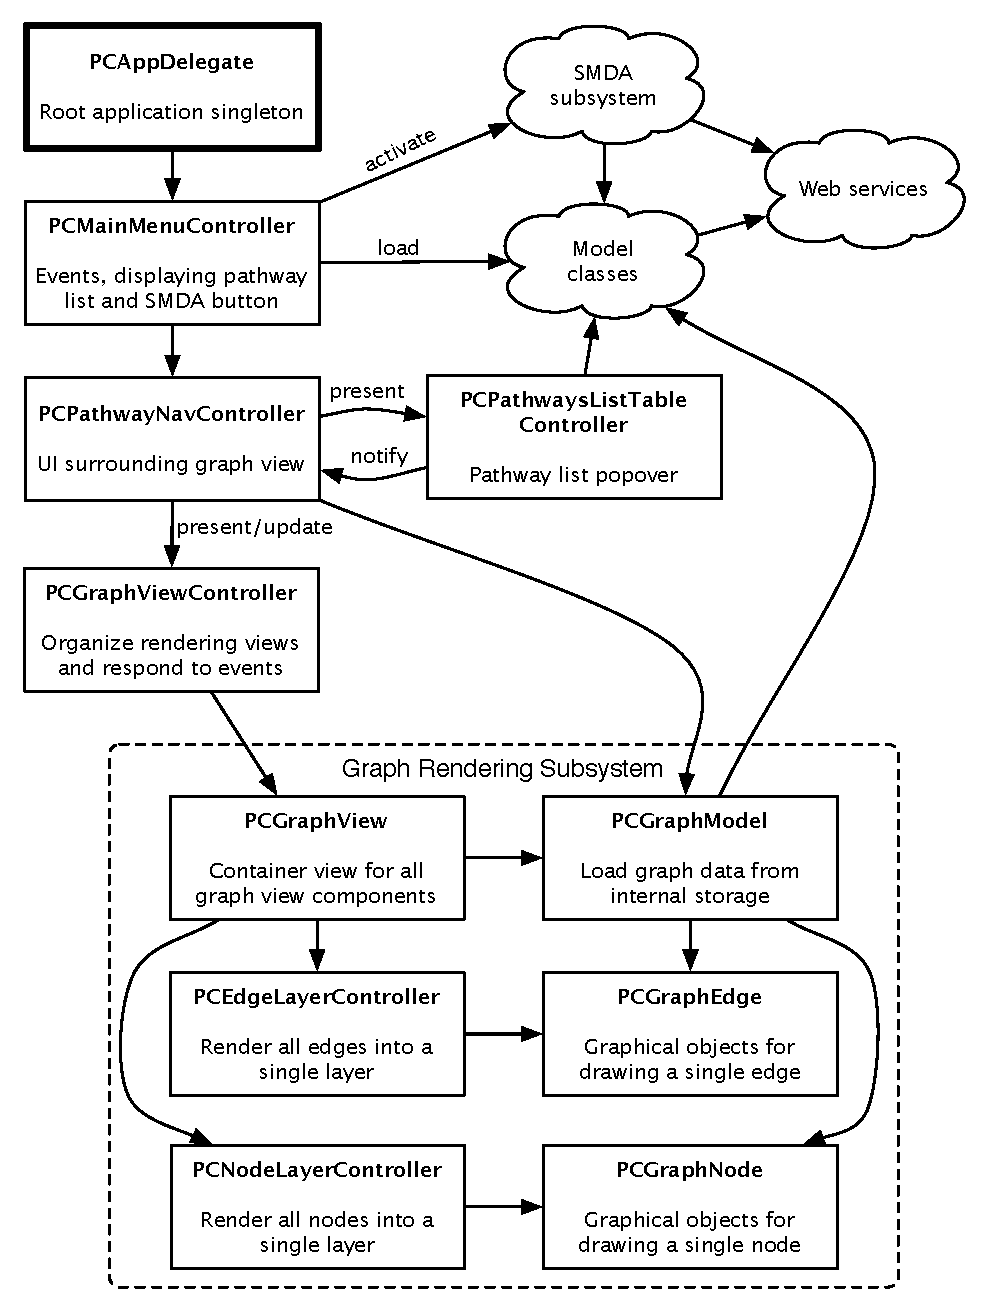
\includegraphics[width=\textwidth]{maw/figures/components.pdf}}
    \caption{\label{fig:maw_components} Components of the architecture}
\end{figure}

\begin{figure}[htbp]
    \center{
        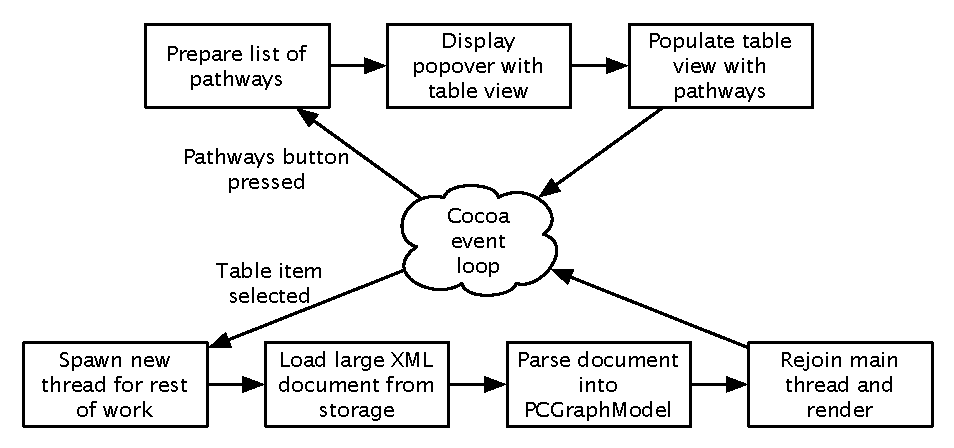
\includegraphics[width=\textwidth]{maw/figures/controlflow.pdf}}
    \caption{\label{fig:maw_controlflow} Control flow for displaying graphs}
\end{figure}

\begin{figure}[thbp]
    \center{
        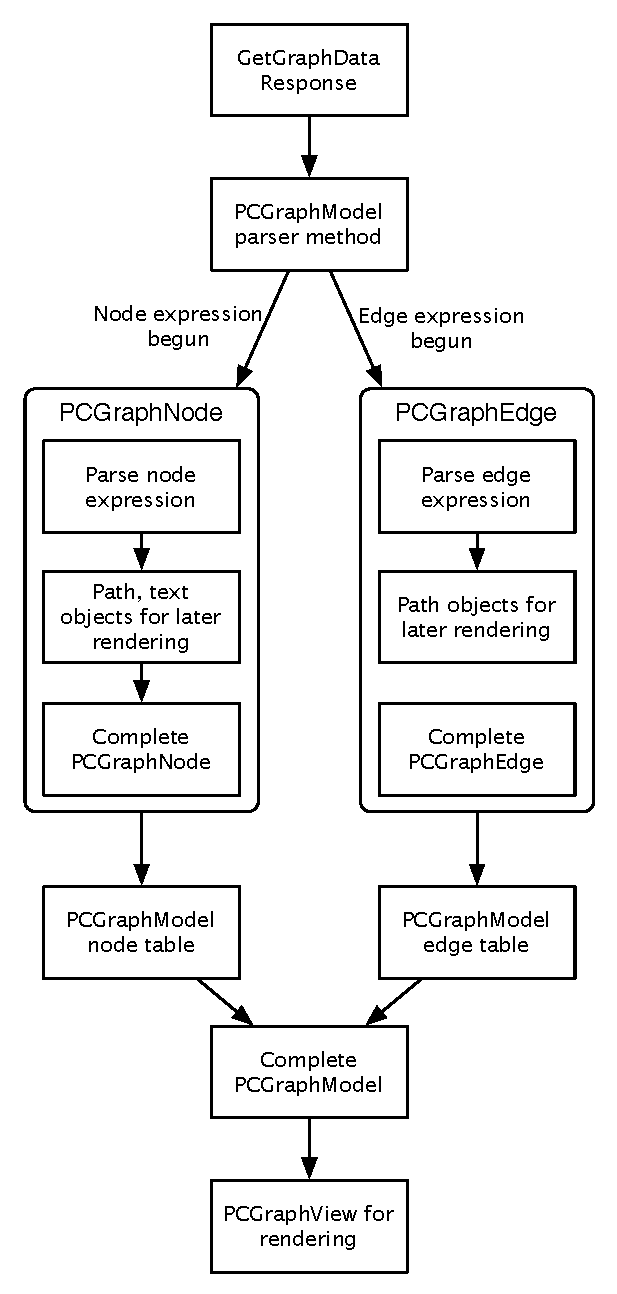
\includegraphics[width=4in]{maw/figures/dataflow.pdf}}
    \caption{\label{fig:maw_dataflow} Data flow for graph data}
\end{figure}
